%!TEX root = ../../csuthesis_main.tex
\chapter{深度强化学习理论基础}

\section{强化学习模型}

在强化学习(RL)的领域,它也被称为增强学习或再励学习。该领域的研究主要集中在查看代理与环境之间的交互。在这样做时,代理人选择由环境提供的有关代理行为的信息,代理根据由环境提供的行为信息来做出决策并更好地学习。这是代理与环境之间最大的交互。其本质是代理与环境交互以创建动作并实施策略。选择这些行动和方法的依据是代理根据环境数据评估系统的状态和性能。强化学习算法无需对问题进行建模或熟悉环境。重点是数据研究,以确保代理和环境之间有更好的互动。良好的数据可以让代理的行动和方法也得到优化和改进。在激励培训的背景下,了解代理与了解一个人的学习过程非常相似。代理通过与环境的互动获得适当的奖励,然后通过结合上述奖励和惩罚,代理可以获得适当的奖励。通过反复尝试和不断学习,代理可以逐渐找到最合适的表现方式,从而实现全局最优。这种试错学习的过程使得代理能够逐步提高其在特定环境中的表现和适应能力。

\subsection{马尔科夫决策过程}


\begin{figure}[hbt]
	\centering
	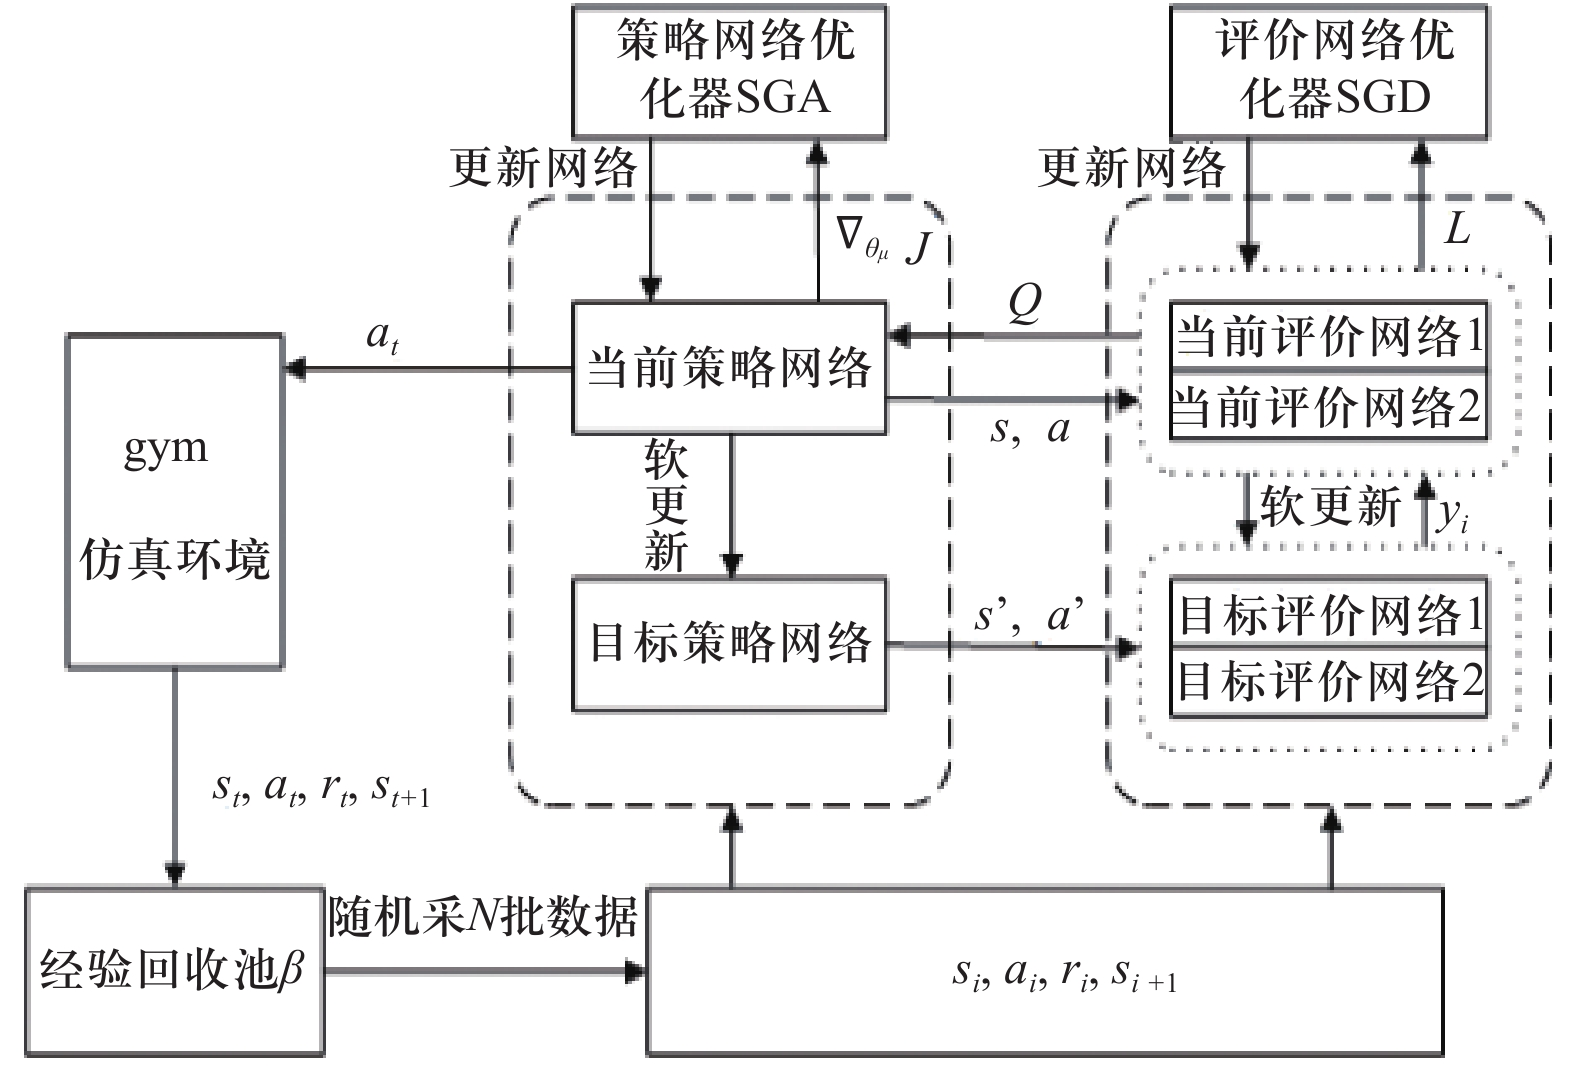
\includegraphics[width=\linewidth]{基于 MDP 的强化学习结构.jpg}
	\caption{基于 MDP 的强化学习结构}
	\label{f.example}
\end{figure}

如果一个系统的状态信息中包含了大量的历史信息,并且不需要提供任何信息,就可以通过结合当前状态来推断出未来的状态,那么这样的状态特性通常被称为马尔可夫特性。结合前面提到的代理与环境的紧耦合,本质上环境的状态是与当前动作紧密相关的,与情境紧密相关的。根据强化学习问题,可以创建马尔可夫决策过程(MDP)\cite{garcia2013markov}。详细流程如上图2-1所示。

智能体获取状态信息,把上述信息当成是输入,结合上述信息,科学选择动作,完成输出。结合动作结果得到相应的奖励,进一步得到未来动作。所以,结合马尔科夫决策过程<$S,A,P,R,$r>
对这一过程进行界定与表述。

首先,需要定义状态。状态是代理接收到的信息,它会对其下一步行动的选择产生一定的影响。状态集群$S$={${s_{1}}$,${s_{2}}$,...,${s_{t}}$}可以由一个或多个动态层组成,通常处理传感器检测到的信息。动作空间$A$={${a_{1}}$,${a_{2}}$,...,${a_{t}}$}表示代理可以选择的动作集合,即它在当前动作中可以选择的所有动作。转移概率表示从当前状态到下一个状态的动作的可能性。如果满足马尔可夫条件,转移概率可以表示为:

\[
P(s_{t+1} \mid s_t, a_t) = P(s_{t+1} \mid s_t, a_t, s_{t-1}, a_{t-1}, \ldots)
\]

奖励函数是一个特定的标量函数,表示在给定状态下应用环境动作后获得的回报值。奖励函数的设计基于状态信息,并影响代理算法参数的评估和优化。折扣因子(也称为折现率)用于加权影响当前和未来回报的因素,从而可以全面分析未来的影响因素。

\begin{figure}[hbt]
	\centering
	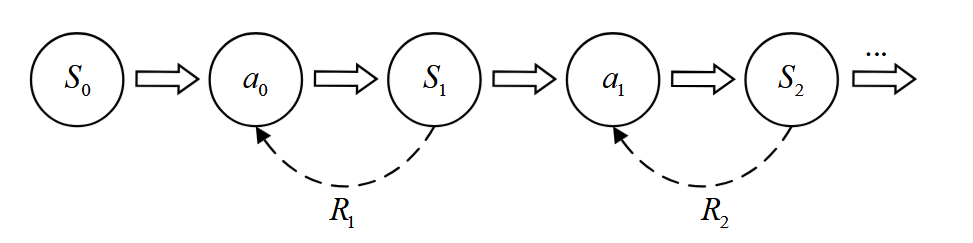
\includegraphics[width=\linewidth]{马尔可夫动态过程.png}
	\caption{马尔可夫动态过程}
	\label{f.example}
\end{figure}

MDP动态传输方案如上图2-2所示。提供者根据有关当前状态的信息选择操作,然后将操作返回给环境。环境做出反应,创造新的情况并创造有价值的回报。随着代理不断与环境交互,学习持续进行,直到到达最后阶段。代理与环境交互以执行最佳策略并最大化总奖励。 MDP 最重要的概念之一是折扣率。它代表未来收益的折现值,即两个不同时间(两个)状态下未来利润的价值之差。

然而,MDP 通信模型基于一个隐含的假设,即代理可以完全访问所有可用信息。然而,在现实情况下,例如对于坦克决策,智能代理可以使用传感器监视环境,因此它无法获取完整的信息并且无法应用 MDP 假设。当代理观察环境时,噪音可能会分散注意力,因此接收到的信息只是实际环境信息的一部分。

本文假设转移概率收敛于马尔可夫过程,这意味着未来状态仅描述当前状态和采取的行动,而不是过去的状态。然而,在高级场景中,传感器提供的有限信息意味着我们无法获得无限的状态信息。因此,从状态空间到存储单元的遍历方式有多种,这使得存储无法满足马尔可夫链的条件。

为了解决这个问题,研究人员提出了几种方法。例如,Shani\cite{shani2013survey}等人开发了一个全面的马尔可夫过程来解释代理和环境之间产生的所有相互信息,假设最初的观察和行动满足马尔可夫特性。

\begin{figure}[hbt]
	\centering
	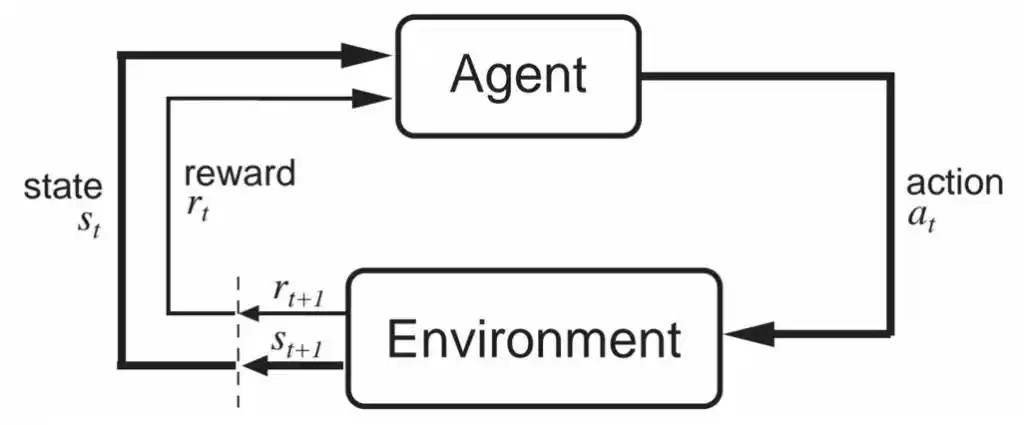
\includegraphics[width=\linewidth]{基于 POMMDP 的强化学习结构.jpg}
	\caption{基于POMMDP的强化学习结构}
	\label{f.example}
\end{figure}

上图2-3给出的是环境同代理交互循环关系,收到观察结果以后代理通过采取动作,同环境之间迭代交互,但代理并非了解真实状态信息。

\subsection{价值函数与策略}


强化学习有两个基本组成部分:财务绩效和策略。两者在算法的设计和优化中都发挥着重要作用。虽然奖励的当前值可以提供有关当前事态的信息,但它仅反映即时奖励,而不能完全预测当前决策的未来结果。因此,衡量一个行动的利弊,必须考虑其后果。在强化学习算法中,成本函数是用于确定给定情况下奖励的预期值的重要参数。这一思想通常以两个函数的形式实现:交易价值函数(Q函数)和状态价值函数(V函数)。后者通常表示为从当前状态到结束状态的期望奖励值,而效用价值函数描述的是执行某项任务后从当前状态到结束状态的奖励的期望值。通过这两项任务,操作员可以更深入地探索环境中的各种物体和行为。

基于这些定义,可以理解状态V的值对代理从当前状态到最终状态所获得的平均工资有直接的影响。当代理做出决策时,他或她倾向于选择能够带来更多价值的任务,以找到最佳的奖励平衡。因此,通过改进成本函数,算法可以在决策过程中变得更加智能和高效,从而提高生产力和项目完成速度。

给定一个状态,就会生成相关的策略约束,并且可以使用独立策略(例如,接近高斯分布)来选择所有点的约束动作。在给定场景中,用户以任意概率分布选择最佳选项。RL的目标是找到使所有人的利润最大化的最优解,如下式所示:

\[
G_t = R(s_t, a_t) + \gamma R(s_{t+1}, a_{t+1}) + \gamma^2 R(s_{t+2}, a_{t+2}) + \ldots + \gamma^k R(s_{t+k+1}, a_{t+k+1})
\]
\[
= \sum_{k=0}^\infty \gamma^k R(s_{t+k+1}, a_{t+k+1})
\]

\subsection{贝尔曼方程}

为了改进学习数据,状态值和交换率函数是贝尔曼方程的解,可以将其分解为各种问题,并可以作为方程获得良好的解\cite{franccois2018introduction}。计算采用两点,旨在达到理想的平衡。

(1) 贝尔曼期望方程

\[
V_{\pi}(s) = E_{\pi} \left[ G_{t+1} \mid s_{t} = s \right]
\]
\[
= \mathbb{E}_x \left[ R_{t+1}(s_t, a_t) + \gamma R_{t+2}(s_{t+1}, a_{t+1}) + \gamma^2 R_{t+3}(s_{t+2}, a_{t+2}) + \ldots \ \middle| \ s_t = s \right]
\]
\[
= \mathbb{E}_{\pi} \left[ R_{t+1}(s_t, a_t) + \gamma \left( R_{t+2}(s_{t+1}, a_{t+1}) + \gamma R_{t+3}(s_{t+2}, a_{t+2}) + \ldots \right) \ \middle| \ s_t = s \right]
\]
\[
= \mathbb{E}_{\pi} \left[ R_{t+1}(s_t, a_t) + \gamma G_{t+1} \ \middle| \ s_t = s \right]
\]
\[
= \mathbb{E}_{\pi} \left[ R_{t+1}(s_t, a_t) + \gamma V(s_{t+1}) \ \middle| \ s_t = s \right]
\]

根据上述公式,对${V}$进行分解处理以后:当前环境下的立即回报值和下一时刻状态值函数可以被我们清晰的看到。

继续进行同样分解${Q}$,可以得到下式:
\begin{align*}
	\underline{Q}_\pi(s) &= \underline{E} \Big[ G_{t+1} \ \Big| \ S_t = s, A_t = a \Big] \\
	&= \underline{E} \Big[ R_{t+1}(s_t, a_t) + \gamma \underline{Q}_\pi(s_{t+1}) \ \Big| \ S_t = s, A_t = a \Big]
\end{align*}

上述表达式中,由于策略$\pi$的影响,可以计算出所有可能性的对应状态值函数的值的为
Q值与$\pi$的乘积的和。如下式所示:

\[
V_{\pi}(s) = \sum_{a \in A} \pi(a|s) Q_{\pi}(s,a) = \mathbb{E}_{a \sim \pi(a|s)} \left[ Q_{\pi}(s,a) \right]
\]

类似的还有下式:

\[
\underline{O}_{\pi}(s, a) = R(s, a) + \gamma \sum_{s' \in S} p(s' \mid s, a) V_{\pi}(s')
\]

(2) 贝尔曼最优方程

此方程是针对两大值函数的内在联系的全面表述,目的是从中挑选出策略对应的最大值
函数,即为最优值函数$V^*(s)$:

\[
V^*(s) = \arg\max_{\pi} V_{\pi}(s), \quad s \in S
\]

同理可得到,最优动作值函数$Q^*(s,a)$:

\[
Q^*(s, a) = \arg\max_{\pi} Q_{\pi}(s, a), \quad s \in S
\]

依据上述两式可得到$V^*(s)$和$Q^*(s,a)$的直接关系式:

\[
V^*(s) = \arg\max_{a} Q^*(s, a)
\]
\[
Q^*(s, a) = R(s, a) + \gamma \sum_{s' \in S} p(s' \mid s, a) V^*(s')
\]

在离散情况下,设置强化学习任务是以有限状态集为依托的,能够获取不同状态s对应
的$V(s)$函数,或$(s,a)$对应的$Q(s,a)$函数。通过计算出$V(s)$,实施更新迭代,结合策略,确定值函数,进而进行评估。再结合上述式子便可以推导出下列式子:

\begin{align*}
	V_{\pi}(s) &= \sum_{a \in A} \pi(a \mid s) Q_{\pi}(s, a) \\
	&= \sum_{a \in A} \pi(a \mid s) \left( R(s, a) + \gamma \sum_{s' \in S} P(s' \mid s, a) V_{\pi}(s') \right)
\end{align*}

针对MDP问题,求出值函数,获取最佳控制策略,必定能够得到最优策略。想要获取
最大策略$\pi^*$,利用最大的$Q^*(s,a)$函数,可以获取最优策略:

\begin{align*}
	\pi^*(a \mid s) &= \arg\max_{a \in A} Q^*(s, a) \\
	&= \arg\max_{a \in A} \left( R(s, a) + \gamma \sum_{s' \in S} p(s' \mid s, a) V^*(s') \right)
\end{align*}

\section{深度神经网络}

在神经网络中,深度神经网络 (DNN) 系统是一个复杂的多层系统,其中许多节点具有多个神经元,通过连接权重传输和处理信息。图 2-4 显示了一个典型的深度神经网络 (DNN) 架构,它由几个隐藏层和一个输出层组成。每个隐藏层和派生层都包含若干个节点,每个节点都与前一层的所有节点相连,并有一定的权重和偏移量。

\begin{figure}[hbt]
	\centering
	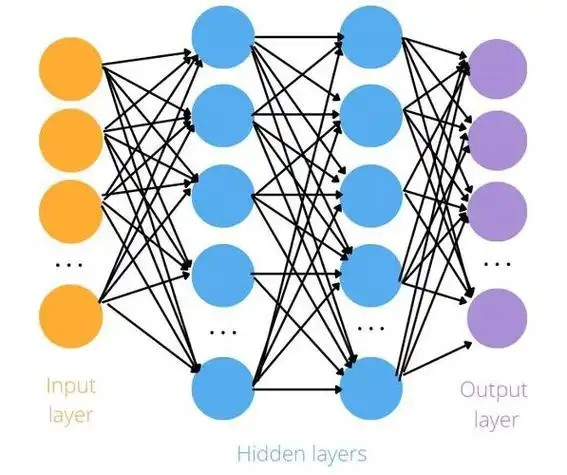
\includegraphics[width=\linewidth]{深度神经网络结构.jpg}
	\caption{深度神经网络结构}
	\label{f.example}
\end{figure}

对于高阶神经网络,权重是归一化的,变分参数也是归一化的。然而,损失函数也代表了相应的误差。一般来说,线性回归问题基于平方误差,平方误差被视为损失函数,解释为:

\[
\text{loss}(Y, \hat{Y}) = \frac{1}{N} \sum_{i=1}^{N} \left( \hat{\mathcal{V}}_i - \mathcal{V}_i \right)^2
\]

其中,训练样本数为N,预测值为$\hat{Y}$,实际值为$Y_(i)$。在训练过程中,输入数据可以来回传递以获得所有层的输出数据。这代表了分层网络中神经元的误差。

在深度神经网络的训练过程中,反向传播算法扮演着至关重要的角色。一旦通过前向传
播获得了各层的输出,就可以利用反向传播来计算每一层神经元的误差,从而进一步计算关
于权重和偏置参数的梯度。

\subsection{卷积神经网络}

在CNN中,卷积提取图像的局部特征,并且卷积可以降低特征图的维度,从而可以减少特征的数量和网络的大小。此外,知识库也得到了显著改善。同时,在网络中采用权重分配的方法可以显著减少参数数量,显著增加模型的泛化效率,显著提高模型的学习效率。

总体而言,该算法的使用提高了深度学习在成像任务中的表现。该模型可用于大规模图像数据的处理。此外,计算机视觉领域取得了长足的进步,并且发展迅速。

\begin{figure}[hbt]
	\centering
	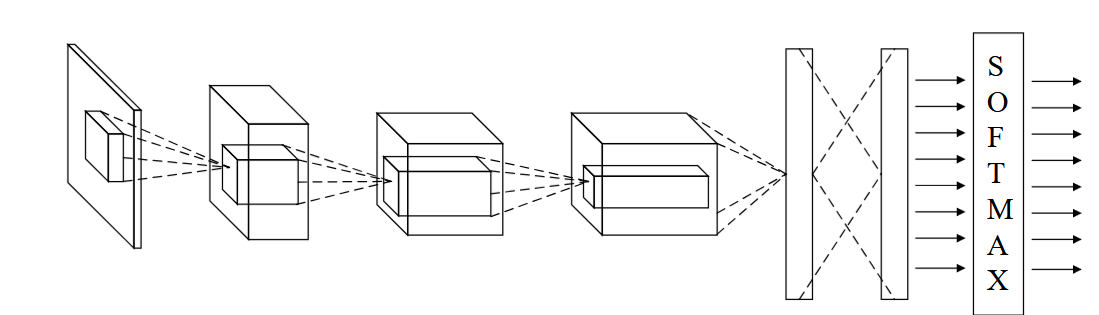
\includegraphics[width=\linewidth]{图像分类卷积神经网络结构示意图.png}
	\caption{图像分类卷积神经网络结构示意图}
	\label{f.example}
\end{figure}

图2-5展示了卷积神经网络的基本结构,它由多个卷积层和池化层组成,对输入图像的特征提取和降维起着关键作用。降低卷积特征图的维度可以减少参数数量并降低计算复杂度,同时保留图像的重要特征。

经过一系列折叠和汇总操作后,特征图被发送到全连接层,该层组合每个特征图中的特征信息,并使用非线性函数对其进行操作,以捕获特征之间的复杂交互。全连接层的输出被送到Softmax层,Softmax层使用似然法对结果进行处理,得到各个类的概率分布,从而深入了解输入图像的分类。此类网络结构具有强大的特征提取和分类能力,在图像分析、目标检测等任务中能够取得优异的效果。在训练过程中,反向传播算法可以让网络自动学习特征的最佳表示,从而对图像进行准确的分类。在卷积神经网络中,常见的输入信号是 RGB 图像,其中每个像素包含来自三个通道的信息:红色、绿色和蓝色。

例如,VGG-16 模型\cite{simonyan2014very}使用的输入数据是 224×224×3 的 RGB 图像。输入数据一旦送入网络,就必须经过多层卷积和池化来降低其维度。在这个例子中,卷积层由两条路径组成:一条是具有多层的卷积层,另一条是最大池化层。一般情况下每个卷积层的卷积核大小为3*3,经过一个大的合并层进行特征提取,减少特征图尺寸。执行这些操作允许网络从输入图像中提取局部重要特征。在卷积过程中,每个卷积核对输入图像进行加权和局部空间的组合,得到神经元的输入。为了显著提高交换网络的非线性能力,应考虑采用更高的输入值作为非线性激活函数,其中ReLU激活函数被广泛使用。这样就可以得到功能图所有区域的输出值。聚合方法采用2×2的最大聚合,即选取每个局部2×2区域内出现的最大值,在保留重要性的前提下,显著降低了数据对象的维度。

\begin{figure}[hbt]
	\centering
	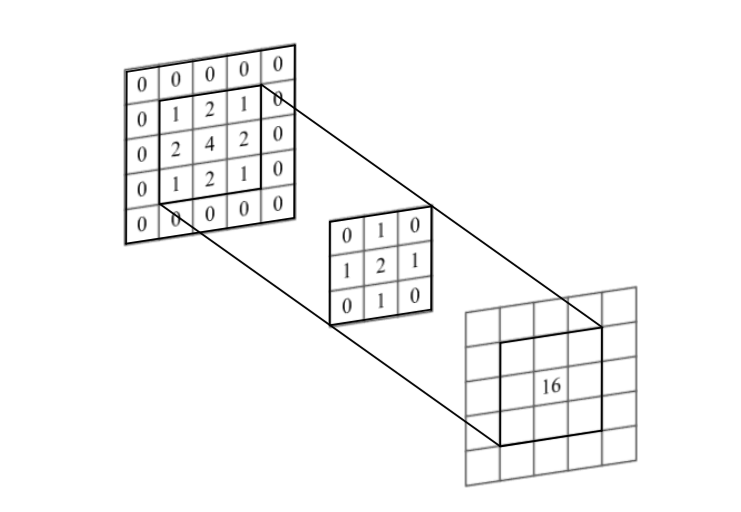
\includegraphics[width=\linewidth]{卷积计算示意图.png}
	\caption{卷积计算示意图}
	\label{f.example}
\end{figure}

在 2016 年,国内学者何凯明总结出 ResNet 残差网络\cite{he2016deep},在这之中,将残差单位加入进
来,不使用其它参数时,可以实现前向反馈神经网络训练。这一单元结构具体见下图2-7。

\begin{figure}[hbt]
	\centering
	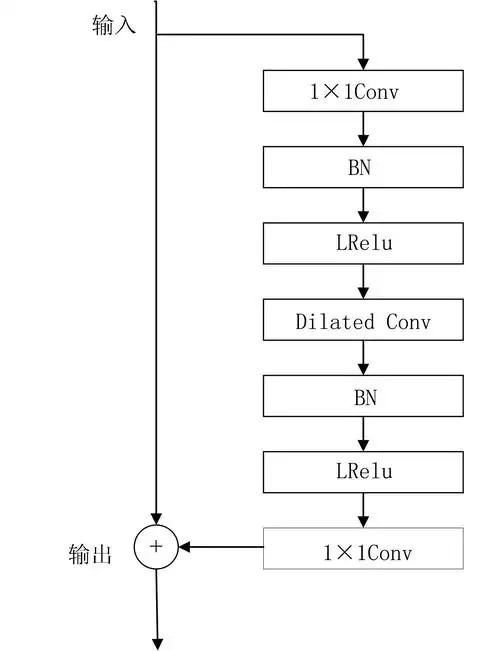
\includegraphics[width=\linewidth]{残差单元.jpg}
	\caption{残差单元}
	\label{f.example}
\end{figure}

在执行语义分割等任务时,卷积神经网络需要处理大量像素级的数据,这使得网络变得复杂且深层。虽然这些深度学习方法可以提供更好的性能和准确的结果,但它们在训练时间和估计方面会带来很大的开销。特别是在实时应用和资源受限的环境中,例如移动设备或嵌入式系统,深度神经网络的设计需要特别注意网络复杂性和计算约束。大型网络将无法在这些设备上运行,也无法满足实际需求。因此,在构建深度神经网络的过程中,除了选择合适规模的网络之外,还需要考虑网络深度。适当的深度可以在保持效率的同时,减少间隙数量和计算复杂度,从而提高网络的效率和效果。这将需要网格修剪、参数共享和模型压缩等技术来减少网格尺寸而不牺牲性能。

\subsection{循环神经网络}

循环神经网络 (RNN)\cite{zaremba2014recurrent}可用于避免在某些会话中运行这些任务时出现非目标计算。它主要由多层循环神经网络组成,如下图所示。通过求解连续序列中的单元,可以得到一个线性神经网络的结构。数据从前向后流动,单元运行后得到的结果用作下一个单元的输入。线性迭代操作按此顺序执行,结构如图2-8所示。

\begin{figure}[hbt]
	\centering
	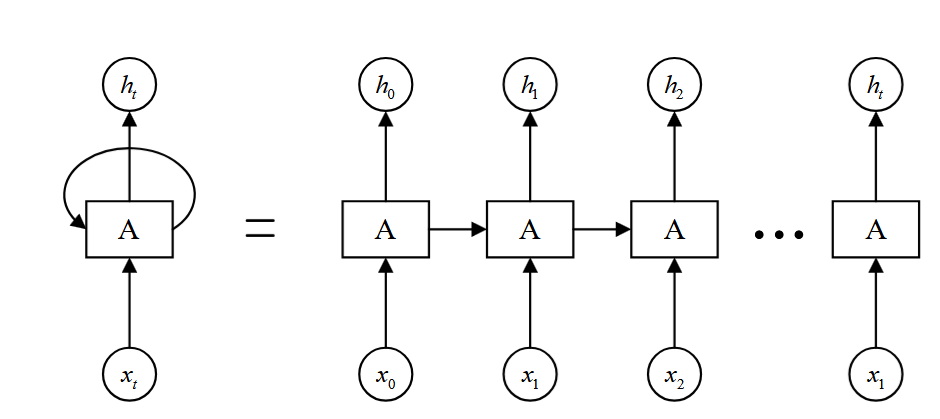
\includegraphics[width=\linewidth]{基础循环神经网络单元.png}
	\caption{基础循环神经网络单元}
	\label{f.example}
\end{figure}

在循环神经网络的实际实现中,也会出现一些难以有效避免的问题。例如,连接数量的不断增加会导致神经网络的增长,并且这种网络的增长无法得到有效的抑制。因此,它在深度联想学习中的作用尚未完全了解。 LSTM\cite{hochreiter1997long}的出现为解决这一问题提供了新的思路。它由三部分组成:输入阀、输出阀和忘记阀。这三个门的加入,使得我们可以忘记不需要记住的信息,保留需要记住的信息,有效地解决了信息长期保留的问题。网络结构如图2-9所示。

\begin{figure}[hbt]
	\centering
	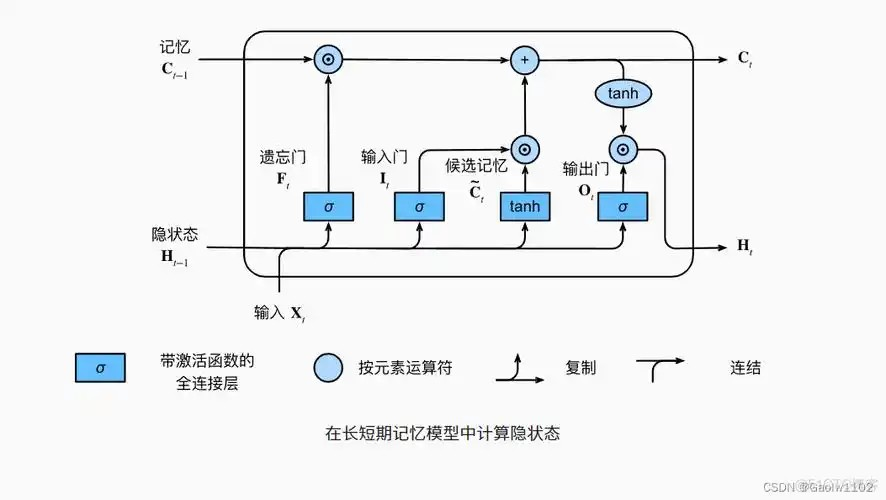
\includegraphics[width=\linewidth]{长短时记忆网络.jpg}
	\caption{长短时记忆网络}
	\label{f.example}
\end{figure}


